\documentclass[11pt,twoside,a4paper,BCOR8.25mm,DIV10,headsepline,footsepline,]{scrbook}
%------------------------------------------------------------------------------
%- PAKETE
%------------------------------------------------------------------------------
	%DIN A4
		\usepackage{a4}   
	%Ränder
		\usepackage[lmargin=2.5cm , rmargin=2.5cm]{geometry}

	%Fancy headers
		\usepackage{fancyhdr}
	
	%Sprache einstellen (Inhaltsverzeichnis, ...)
		\usepackage[english,ngerman]{babel} %american,italian,german
	
	%Euro Zeichen
		\usepackage{eurosym}	
		
		\usepackage[bookmarks=true,
					bookmarksopen=true,
   					% Lesezeichen ausgeklappt
					bookmarksnumbered=true,
					colorlinks=false,
				   	%Einf�rbung von Links
					linkcolor=black
					% Linkfarbe: schwarz					
					]
				    % Anzeige der Kapitelzahlen am Anfang der Namen der Lesezeichen
				   {hyperref}
		
	% Vereinfachtes Eingeben von Leerschl�gen hinter Shortcut-Commands
	% Beispiel: \newcommand{\DNA}{desoxyribose nucleid acid\xspace}
		\usepackage{xspace}
	
	%Sortierte Literaturverweise
		\usepackage{cite}
	
	%Grafiken
		\usepackage{float} %Float-Handling mit Schalter H (gleiche Position wie im Skript)
		\usepackage{floatflt}
		%\usepackage{flafter} %Verhindert Figuren vor ihrer ersten Referenz
		\usepackage{placeins} %Barriere f�r Float-Umgebungen erzeugen mit \FloatBarrier
	
	%Verbessertes Beschriften mir div. Optionen
		\usepackage[format=plain,labelsep=colon,labelfont=bf,textfont=it]{caption}
	
	%Zusaetzliche Symbole und Schriften (ams: american mathematical soc)
		\usepackage{amssymb}
		\usepackage{amsmath}
		%\usepackage{amstext}
		%\usepackage{amsfonts}
		%\usepackage{amsbsy}
		%\usepackage{amscd}
		%\usepackage{latexsym}

	%Text Companion fonts which provide many text symbols (such as baht, bullet, copyright, musicalnote, onequarter, section, and yen) in the TS1 encoding.
		\usepackage{textcomp}
	
	%Drehen von Text, Tabellen, Seiten
		%\usepackage{rotating}
	
	%including graphics files, rotating parts of a page, and scaling parts of a page
		\usepackage{graphicx}
	
	%Nice drawing package
		%\usepackage{tikz}               
	
	%besserer eps import: \eps import ERSETZEN durch \epsfig
		\usepackage{epsf}
	
	%Farbunterst�tzung (ausserhalb der Bilder)
		\usepackage{color}
	
	%Postcript einbinden, wobei Text ersetzt werden kann
		%\usepackage{psfrag}
	
	%F�r den Index
		\usepackage{makeidx}
		\makeindex %Muss vor begin{document}, sonst passiert nix
	
	%Erleichterungen f�rs Deutsche inkl Silbentrennung
		%\usepackage{german}
	
	%Ensure minimal spacing of table cells (http://www.ctan.org/tex-archive/help/Catalogue/entries/cellspace.html)
		\usepackage{cellspace}
	
	%Direkte Eingabe von Umlauten mit Angabe von Schriftsatz
	%in Kombination mit 'german' sind jetzt � direkt erlaubt!
		\usepackage[utf8]{inputenc}
	
	%Source code Listings 
		\usepackage{listings}
	
	%Darstellung von Algorithmen
		\usepackage{algorithm}
		\usepackage{algorithmic}
	
	%Subfigures
		\usepackage{subfigure}

%-- Fieser Hack f�r Subfigures (braucht man, um lstlistings im Subfigures zu nutzen)
\newbox\subfigbox
\makeatletter
\newenvironment{subfloat}
{\def\caption##1{\gdef\subcapsave{\relax##1}}%
\let\subcapsave\@empty
\setbox\subfigbox\hbox
\bgroup}
{\egroup
\subfigure[\subcapsave]{\box\subfigbox}}
\makeatother
	
	%Automatically adds the bibliography and/or the index and/or the contents, etc., to the Table of Contents listing.
		%\usepackage[nottoc]{tocbibind} %,notlot,notlof
	
	%St Mary Road symbols for theoretical computer science.
		%\usepackage{stmaryrd}
	
	%URL Darstellung
		\usepackage{url}


	%PDF und Standard Latex Unterscheidung
		\usepackage{ifpdf} 

	%Fancy verbose environments
		\usepackage{fancyvrb}	

	%Abk�rzungsverzeichnis
		\usepackage{nomencl}
		  \let\abbrev\nomenclature
		  \renewcommand{\nomname}{Abk�rzungsverzeichnis}
		  \setlength{\nomlabelwidth}{.25\hsize}
		  \renewcommand{\nomlabel}[1]{#1 \dotfill}
		  \setlength{\nomitemsep}{-\parsep}
		  \makenomenclature

	  \newcommand{\abk}[2]{#1\abbrev{#1}{#2}}
				
	%With \usepackage{ulem}, you have the following new commands:
		%    * \uline{important} underlined text
		%    * \uuline{urgent} double-underlined text
		%    * \uwave{boat} wavy underline
		%    * \sout{wrong} line drawn through word
		%    * \xout{removed} marked over with //////.
		%    * {\em phasized\/} and \emph{asized} In LaTeX, by default, these are underlined; use \normalem or [normalem] to restore italics
		%    * \useunder{\uwave}{\bfseries}{\textbf} use wavy underline in place of bold face 
		%Note that this package changes \em and \emph to be underline. To change this behavior back to normal, use the \normalem command, for example
		%\usepackage{ulem}
		%\normalem
		%\usepackage[normalem]{ulem}

	  %\newcommand{\markup}[1]{\uline{#1}}	

	% package to customize the three basic lists (enumerate, itemize and description) 
	% by means of a set of parameters, and to clone them to define new "logical" lists.
		\usepackage{enumitem}
		\setitemize{enumsep=-3pt}
		\setitemize{itemsep=-3pt}

	%Definitionen
		\usepackage{theorem}
		\newcounter{theorem}
		\newtheorem{definition}[theorem]{Definition}

	%Zitate
		\newcounter{quotectr}
		\newtheorem{myquote}[quotectr]{Zitat}

%------------------------------------------------------------------------------
%- Layout
%------------------------------------------------------------------------------

	%Tiefe des Inhaltsverzeichnisses und der Nummerierung der Kapitel
		\setcounter{secnumdepth}{2}
		\setcounter{tocdepth}{2}

	%Call this after each chapter to avoid headlines on empty pages
		\newcommand{\chapterfin}{\clearpage{\pagestyle{empty}\cleardoublepage}}
		\newcommand{\sectionfin}{\clearpage{\pagestyle{empty}\cleardoublepage}}

	% Listings schoen machen 
		\renewcommand*\ttdefault{txtt}
	
		\lstset{%
		  breaklines=true,
		  basicstyle=\ttfamily\footnotesize,%
		  moredelim=[is][\fontseries{lt}\bfseries]{|}{|},%
		  captionpos=b,%
		  numbers=left,%
		  tabsize=1,%
		  numberstyle=\tiny,%
		  numbersep=6pt,%
		  frame=lr,%
		  framesep=0pt,%
		  framexleftmargin=5pt,%
		  framextopmargin=0pt,%
		  framexbottommargin=0pt,%
		  xleftmargin=15pt,%
		  xrightmargin=15pt,%
			abovecaptionskip=0pt,%
			belowcaptionskip=-0pt,%
		}	
		
		\lstdefinelanguage{XMLSchema}
			{morekeywords={schema,element,annotation,appinfo,complexType,simpleType,choice,all,sequence},		
			sensitive=true,
%			morecomment=[l]{//},
%			morecomment=[s]{/*}{*/},
			morestring=[b]",
		}
		
		\lstdefinelanguage{ASN1}
			{morekeywords={},		
			sensitive=true,
%			morecomment=[l]{//},
%			morecomment=[s]{/*}{*/},
			morestring=[b]",
		}
		
	
	% Font
	%
	%	Danach muss man die Standardschriftart setzen mit dem Befehl \fontfamily{abr}\selectfont, 
	% der f�r das gesamte restliche Dokument gilt, oder mit {\fontfamily{abr}\selectfont Some Text} 
	% um nur den eingeklammerten Bereich zu betreffen. abr ist die Abk�rzung f�r die Schriftart. Die 
	% h�ufigsten sind ptm (Times), phv (Helvetica), pcr (Courier), pbk (Bookman), pag (Avant Garde), 
	% ppl (Palatino), bch (Charter), pnc (New Century Schoolbook), pzc (Zapf Chancery), put (Utopia ).

	% Sch�nerer tt font:
		%\renewcommand{\ttdefault}{pcr}
		%\selectfont
	
	% Times
		%\usepackage{times}
		
	%	Helvetica
			%\usepackage{helvet}
			%\renewcommand{\familydefault}{\sfdefault}
			%\renewcommand{\familydefault}{phv}
			%\fontfamily{abr}\selectfont
			
	%	Courier
			%\usepackage{courier} \raggedright
			%\renewcommand{\familydefault}{\ttdefault}
	
	% Absatzformatierungen:
	% Keeps the distance between paragraphs constant
		\setlength{\parskip}{1.5ex plus 0.0ex minus 0.0ex}
		\setlength{\parindent}{0pt}
	
	% Modify the placement of figures: from faq source: You can adjust the cut-off value if you like, 
	% but it makes no sense to go higher than .95 (LaTeX's default value is only .5). Also, the first 
	% 3 values should be equal, and the last should be 1 - \floatpagefraction.  Otherwise, you are 
	% likely to get floats flushed to the end. 
		\renewcommand{\floatpagefraction}{0.9}
		\renewcommand{\topfraction}{0.9}
		\renewcommand{\bottomfraction}{0.9}
		\renewcommand{\textfraction}{0.1}
		\renewcommand{\textfloatsep}{5mm}
	
	% Zeilenabstand
		\renewcommand{\baselinestretch}{1.25}

	% Fancyheaders 	
		\fancyhf{} % Delete all fields
		%\fancyhead[EL,OR]{\thepage}
		\fancyhead[EL]{\nouppercase{\leftmark}}
		\fancyhead[OR]{\nouppercase{\rightmark}}
		\fancyfoot[EL,OR]{\thepage}	
		
	% Itemize look and feel
		\renewcommand{\labelitemi}{\rule[+0.9mm]{2.7pt}{2.7pt}}
		\renewcommand{\labelitemii}{--}
		%\renewcommand{\labelitemiii}{}
		%\renewcommand{\labelitemiv}{\#}	

	% Floats richtig benennen:
		%\floatname{algorithm}{Algorithm}
		%\renewcommand{\listalgorithmname}{Algorithmen}
		
%------------------------------------------------------------------------------
%- Textbausteine
%------------------------------------------------------------------------------

	%Helpers
		\newcommand{\todo}[1]				{{\em [#1]}\marginpar{{\bf [!!!]}} }
		
		\newcommand{\eigenname}[1]	{{\em #1}}
		
	%Deutsch
		\newcommand{\figref}[1]{Abbildung~\ref{fig:#1}}
		\newcommand{\tabref}[1]{Tabelle~\ref{tab:#1}}
		\newcommand{\equref}[1]{Gleichung~\ref{equ:#1}}
		\newcommand{\chapref}[1]{Kapitel~\ref{cha:#1}}
		\newcommand{\appref}[1]{Anhang~\ref{cha:#1}}
		\newcommand{\secref}[1]{Abschnitt~\ref{sec:#1}}
		\newcommand{\lstref}[1]{Listing~\ref{lst:#1}}
		\newcommand{\algref}[1]{Algorithmus~\ref{alg:#1}}
		\newcommand{\ssecref}[1]{Unterabschnitt~\ref{ssec:#1}}
		\newcommand{\quoteref}[1]{Zitat~\ref{quote:#1}}

	%Englisch	
		%\newcommand{\figref}[1]		{Figure~\ref{fig:#1}}
		%\newcommand{\tabref}[1]		{Table~\ref{tab:#1}}
		%\newcommand{\equref}[1]		{Equation~\ref{equ:#1}}
		%\newcommand{\algref}[1]		{Algorithm~\ref{alg:#1}}
		%\newcommand{\defref}[1]		{Definition~\ref{def:#1}}
		%\newcommand{\quoteref}[1]	{Quote~\ref{quote:#1}}
		
		%\newcommand{\chapref}[1]	{Chapter~\ref{cha:#1}}
		%\newcommand{\appref}[1]		{Appendix~\ref{cha:#1}}
		%\newcommand{\secref}[1]		{Section~\ref{sec:#1}}
		%\newcommand{\ssecref}[1]	{Section~\ref{ssec:#1}}
		%\newcommand{\sssecref}[1]	{Section~\ref{sssec:#1}}
		
	% REDEFINE UGLY STUFF
		\renewcommand{\leq}		{\leqslant}
		\renewcommand{\geq}		{\geqslant}
		\renewcommand{\epsilon}	{\varepsilon}
		\newcommand{\musec}		{$\mu sec$\xspace}
		\newcommand{\muW}		{$\mu W$\xspace}
		\newcommand{\plusminus}	{$\pm $\xspace}
	
%------------------------------------------------------------------------------
%- Worttrennung
%------------------------------------------------------------------------------
	
	%\hyphenation{Ge-samt-ozon}	
	\hyphenation{name-space}	
	\hyphenation{name-spaces}	
	\hyphenation{ge-samten}	
			
%------------------------------------------------------------------------------
%- Grafiken
%------------------------------------------------------------------------------

	\ifpdf
	  \DeclareGraphicsExtensions{.jpg,.pdf,.png}   % for pdftex driver
	\else
	  \DeclareGraphicsExtensions{.eps}             % for dvips driver
	\fi
	
	% Vereinfacht die Einbettung von Grafiken
	% Beispiel: \myfig[5cm]{psdatei}{�bersicht �ber das Gesamtsystem}
	\newcommand{\myfig}[3][\columnwidth]
	{
	 \begin{figure}[htbp]
		 \begin{center}
			 \includegraphics[width=#1]{img/#2}
			 \caption{#3}
			 \label{fig:#2}
		 \end{center}
	 \end{figure}
	}
	
	\newcommand{\myfigtwo}[4][\columnwidth]
	{
		 \begin{figure}[htbp]
				\begin{center}
				  \mbox
				  {
				    \subfigure[#2] 
				    { \includegraphics[width=.45\columnwidth]{img/#1-a} \label{fig:#1-a} } 
				    \quad
				    \subfigure[#3]
				    { \includegraphics[width=.45\columnwidth]{img/#1-b} \label{fig:#1-b} }
			    }
				  \caption{#4}
					\label{fig:#1}
				\end{center}
			\end{figure}
	}
	
	\newcommand{\myfigthree}[5][\columnwidth]
	{
		 \begin{figure}[htbp]
				\begin{center}
				  \mbox{
				    \subfigure[#2]
				    {
				    	\includegraphics[width=.3\columnwidth]{img/#1-a}
				    	\label{fig:#1-a}
				    } 
				    \subfigure[#3]
				    {
							\includegraphics[width=.3\columnwidth]{img/#1-b}
				    	\label{fig:#1-b}
				    }
				    \subfigure[#4]
				    {
							\includegraphics[width=.3\columnwidth]{img/#1-c}
				    	\label{fig:#1-c}
				    }
			    }	
				  \caption{#5}
					\label{fig:#1}
				\end{center}
			\end{figure}
	}
	
	\newcommand{\myfigfour}[6][\columnwidth]
	{
		 \begin{figure}[htbp]
				\begin{center}
				  \mbox
				  {
				    \subfigure[#2] 
				    { \includegraphics[width=.45\columnwidth]{img/#1-a} \label{fig:#1-a} } 
				    \quad
				    \subfigure[#3]
				    { \includegraphics[width=.45\columnwidth]{img/#1-b} \label{fig:#1-b} }
			    }
				  \mbox
				  {
				    \subfigure[#4] 
				    { \includegraphics[width=.45\columnwidth]{img/#1-c} \label{fig:#1-c} } 
				    \quad
				    \subfigure[#5]
				    { \includegraphics[width=.45\columnwidth]{img/#1-d} \label{fig:#1-d} }
			    }
			    
				  \caption{#6}
				\label{fig:#1}
				\end{center}
			\end{figure}
	}
	


%Um die Abkuerzungen zu ermoeglichen:
% 	makeindex.exe thesis.nlo -s nomencl.ist -o thesis.nls
%   als Postprocessor in Texniccenter einrichten

% Nette Hinweise zum LaTexen einer Diss: 
% - http://iacweb.ethz.ch/en/various/Mittelbau/disslatex.html
% - http://www.zib.de/pfetsch/Diss-Styles/
% - http://www2.informatik.hu-berlin.de/~nlohmann/arbeit/koma.html

% Hiermit kann man festlegen, dass immer nur ein bestimmter Teil übersetzt wird
%\includeonly{1-einleitung}
\definecolor{orange}{RGB}{255,204,102}
\begin{document}
\selectlanguage{english}
\frontmatter

%---------------------------------------------------------------------------
% Frontpage
%---------------------------------------------------------------------------
	%---------------------------------------------------------------------------
% Frontpage
%---------------------------------------------------------------------------

\begin{titlepage}

\author{Maximilian Mühlfeld}

\let\footnotesize\small
	\let\footnoterule\relax
	\null
	\vfil
	\vskip 30pt
	\begin{center}
		{\LARGE
		  {
\includegraphics[width=80mm]{Logo_Uni_Luebeck_300dpi.png}
			\\
			\vskip 15pt
			\Large Universität zu Lübeck}\\
			Institute for Robotics and Cognitive Systems \\[2cm]
			{\Large Master Thesis}\\ [1cm]
			An Approach to Solving Object Displacement Problems 
			\par}%
		\vskip 4em
		{\large \lineskip .75em
		\begin{tabular}[t]{c}
			{\Large written by}\\[.5em]
			{\Large Maximilian Mühlfeld (580070)}\\\\
			{\bf Supervisor:}\\[.5em]
			Prof. Dr.-Ing. Achim Schweikard
		\end{tabular}
		\par}%
		\vfill 
		{\large
			Lübeck, \today
			\par}%
	\end{center}
	\par
	% thanks
	\vfil
	\null
\end{titlepage}

%\cleardoublepage

% Erklaerung
\newpage
\vspace*{1cm}
\centerline{\bf Assertion}

\vspace*{1cm}
I assure that the following work is done independently with the use of only stated 
resources.

\vspace*{3cm}
Lübeck, \today 
\newpage

%\vspace*{3cm}
%L�beck, den \today 


%\vspace*{3cm}
%L�beck, den \today 


%\vspace*{3cm}
%L�beck, den \today 

\pagestyle{headings}

%\cleardoublepage

% Kurzfassung und Abstract
\centerline{\bf Abstract}



%
\vskip 2cm
%

%\centerline{\bf Abstract}
%\bigskip
%This thesis in short.

%\cleardoublepage
The scope of this thesis grasps the implementation and testing of algorithms to solve object displacement problems.\\
To achieve this, the search space is divided into multiple cells to reduce its size. Furthermore, instead of calculating the whole space at once, a local approach is used to only calculate the parts needed for the next search step. This needs a wide range of basic geometric and algebraic algorithms for object representation, collision detection and object translation as well as rotation.\\
On the resulting search space a simple and exchangable graph search algorithm is applied, which gives a path in the object space from the
start configuration to the desired target configuration.

%%
%\vskip 4cm
%%
%\centerline{\bf Abstract}
%
%
%
%%
%\vskip 2cm
%%
%
%%\centerline{\bf Abstract}
%%\bigskip
%%This thesis in short.
%
%%\cleardoublepage
%The scope of this thesis is the implementation and testing of algoritms to solve object displacement problems.\\
%To achieve this the search space is divided into multiple cells to reduce its size. Furthermore instead of calculating the whole space at once, a local approach is used to only calculate the parts needed for the next search step. This needs a wide range of basic geometric and algebraic algorithms for object representation, collision detection and object translation/rotation.\\
%On the resulting search space a simple and exchangable graph search algorithm is applied, which will give us a path in the object space from
%start configuration to the desired target configuration.

%---------------------------------------------------------------------------
% Inhaltsverzeichnis
%---------------------------------------------------------------------------
	\tableofcontents
	%\cleardoublepage

%---------------------------------------------------------------------------
% Der eigentliche Inhalt
%---------------------------------------------------------------------------
	\mainmatter
	\pagestyle{fancy}
	
	\lstset{language=Matlab}

	\chapter{Introduction}
\label{cha:Introduction}

\section{Motivation}
\label{sec:Motivation}
\subsection{Path planning in robotics}
In the field of robotics the path planning of an industrial robot can be programmed as a fixed list of movements to be executed. This has multiple drawbacks as for every change in the enviroment the robot needs to manually be reprogrammed.\\
But what if we equip this robot with a camera that detects the shape of objects in the robots enviroment. This would give us a set of objects at certain positions, a robot arm in a starting position and a target where the robots endeffector needs to work. If we would be able to solve this puzzle, we could direct the robot in a different way each time without the actual need to access its software.


\subsection{Geometric riddles in gaming}
Solving geometric riddles is an amazingly fun task for a human. This is the reason many games simply consists of such riddles ranking from easy to hard in difficulty. But even the easiest riddle for a human proposes a big challenge for a simple algorithm that searches trough the possible ways of solving it. Even more complicated is the generation of such riddles. Even for the human brain this task can be exceedingly stressful.\\
 Now, if there would be a possibility to check if such a riddle has a solution, there would be the option to generate them randomly and check for feasibility. This would cast off the necessity for the developers to manually create each riddle. Also the consumers, in this case the players, would have a endlessly stream of new and different riddles to solve.


\section{Idea}
\label{sec:Idea}
For simplification purposes we let our algorithms work on two dimensional object displacement problems. The following riddles shall provide simple examples of the problem:\\

\begin{figure}[h]\centering

\includegraphics[scale=0.1]{circleRiddle.png}
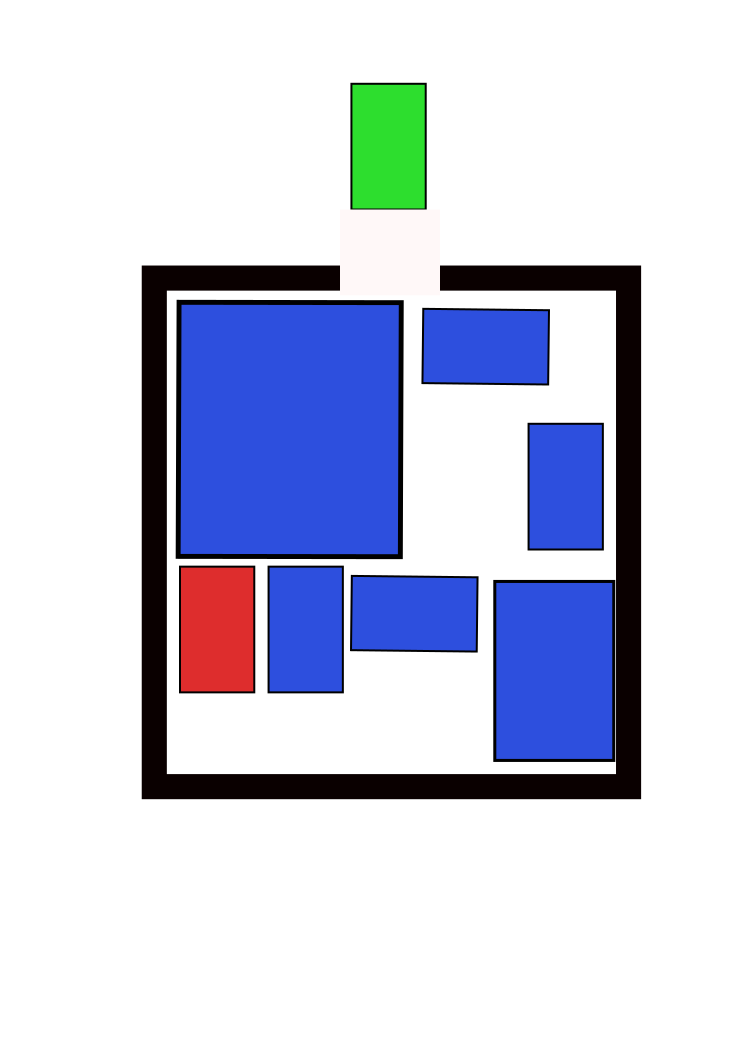
\includegraphics[scale=0.1]{boxRiddle.png}

\includegraphics[scale=0.1]{mixedRiddle.png}
\caption{riddle 1 with circles , riddle 2 with boxes , riddle 3 with 2 half-circles}
\end{figure}

The riddle is solved, if the red box matches the green one. Blue objects are movable and black ones are stationary. The stationary ones will be referred to as rims hereafter.\\
As a human the way to solve those is quite obvious. The first riddle is solved by rotating the blue objects, the second through translation. The third needs both ways to be solved.\\
If we want to solve this with an algorithm, we would need to consider each objects collsision with the other objects and the rim. Also we would need to find a way to express the current configuration consisting of position (x,y) and rotation ($\phi$) and the direction the main object needs to take. A first idea would be to 
\begin{enumerate}
\item Generate all valid configurations per object in regard to the stationary obstacles as a configuration space
\item Create one collision space per object for collision with every other object. 
\item Substract the collision space from the configuration space to get valid space in regard to all obstacles for one object.
\item Divide the space in cells and locate the valid ones.
\item Build a graph out of this starting position by adapting the space after each step.
\item Search in that graph to get a path from start to target point.
\end{enumerate}

The target point would then be a simple configuration vector holding each position of each object. A user defined distance function beetween start and target point in that space can then be used as heuristic in the graph search, e.g. $h(start,target) = || ( x_{start} -  x_{target} , y_{start} - y_{target} ) ||$ .


\section{State of the art}
\subsection{Pathplanning}
The correct answer to the question "Which algorithm is the best for finding the path from start to target" is not as easy as one might suspect. 
It depends on many factors including which structure one searches on ( e.g. graph, net, tree ), what knowledge there is about the current position ( e.g. distance to target ) and what result is needed ( shortest path, "good" path, existence of a path ).\\
For this work the focus is on an algorithm working on a graph with non-negativ edges, an absolute knowledge of the position of the target and the current in a two dimensional coordinate system and a need for a "good" path, not necessarily the shortest. Given these conditions, A$^\star$ is a valid choice. It is a widely used algorithm which calculates a "good" path, not a perfect one. How good the path is depends heavily on the heuristic used. In our case that would be a weighted sum of the distance traveled in steps plus the absolute distance to the target.\\
Another choice could be Dijkstra's algorithm \cite{ComputerScience} itself which is basically A$^\star$ with the heuristic set to constant zero. This would return the shortest path for all calculations. For the named applications from \ref{sec:Motivation} we need the algorithm to be fast, more than to be precise, thus A$^\star$ is the better choice.\\
It should be noted though that the algorithm for pathplanning is exchangable, as long as it is possible to create the graph while searching.

\subsection{Collision detection}
Collision detection in computer science has its home in simulations and computer games as it has in robotics. In this case the focus lies on the way computer games solve collision detection without looking into physical problems that would arise with it.\\
There are a number of ways this has been solved. In a case where there are not that many objects needed to check, pairwise checking is an option. Depending on how the objects are represented, they need to be checked for collision for every step taken. A way around this is to bound objects that lie in a certain proximity of each other together in spheres, where they are only checked in pairs if the spheres containing the objects collide.\\
Also there is a difference in checking if a collision happened, or if it is about to happen. The first option is easy to calculate, because all that is needed is the current position of the objects concerned. The second needs to take into account the movement of all the objects that could collide. In this work, all algorithms know about the movement of the objects so the first option will be neglected.\\
Knowing about the movement allows to check only the objects lying in the way. To determine these obstacles two major algorithms are present.
One way is to start building a spacial binary tree starting from the object, partioning space along the direction of the movement. Until a given spacial size of an end node is reached ( e.g. the bounding box of the moving object) or a obstacle is in the node, the tree keeps on growing. The node directly in front of the last obstacle node would then be choosen as the last safe position to move to.\\
Another way is to build bounding boxes around all object and calculate a plane in space from the moving objects. Then a collision check of this plane with the bounding boxes by post-collision algorithms would yield the distance to the next obstacle in the moving direction. With this information we can place the object just infront on the obstacle without actually colliding with it.\\
This last concept is used and refined to work with convex hulls instead of bounding boxes for calculating the occuring collisions.


\subsection{Applications}
The standard solution in path planning for industrial robots is to hard-code the correct path. This is mostly done by setting a number of safe points on the path from start to target to avoid collision. As a matter of fact, this is a good solution for processing objects where only one simple step for a large quantity is needed. In this scenario only few recalibrations are needed. But if the processed objects change more often, each time the machinist needs to recalibrate the robot. \\
The algorithms from this work would allow for an automatic recalibration of industrial robots without additional supervision.\\
\newline
The automated creation of geometric riddles in computer games is a process widely used in the gaming industry. Not only riddles, whole characters and worlds are created at random.
One of the first famous games that made use of that was Nethack \cite{nethack}. It featured randomized enemy characters in randomized levels. This concept is still in use in todays products. The problem is, that this randomized content is created reversely. For example starting with a valid riddle/ level and then  doing only steps from a certain predetermined set of valid transformations one would reach a randomized mutation which can be used as new content.\\
The way one could create riddles with the algorithms in this work is very different. There would be the option to place "totally" random objects into the riddle and afterwards check for the existence of a solution. "Totally" is relativ because there is still the need to look at the given properties of the riddle. For example if the riddles total space should only be 16x16 units big, putting an object the size of 1x30 units in would not be possible.

 	
	\chapterfin

	\chapter{Enviroment and basics}
\label{cha:enviromentandbasics}

\section{Programming tools}
As the target of this thesis is a mere proof of concept, the programming language of choice is matlab \cite{tool:matlab}. This is a reasobable decision because in the matlab language a huge part of the needed functionality concerning simple mathematical functions is already implemented and easy to use. \\
Pros:
\begin{itemize}
\item easy to use mathematical function
\item fast and easy way to enter data
\item good and simple ways of debugging and locating errors 
\end{itemize}
Cons:
\begin{itemize}
\item slow computation speed
\item needs translation in other language ( e.g. c++ ) for further use
\end{itemize}

As versioning tool git \cite{tool:git} is used together with www.github.com as an open source storage plattform for the resulting code.

\section{Basics}
For better understanding of the following chapters the central mathematical formulas are repeated here.

\subsection{basic vector math} %representation with points
If the objects are represented as a list of corner points, vector math comes in handy when describing the borders of the object.
Lets say we have a simple object A defined by the following list:
\begin{align*}
A = 	&( 0 , 0 ;2 , 0 ;2, 2; 0, 2)	
\end{align*}

Each pair x,y defines one corner of A and the points are ordered to travel along the border of A counterclockwise.
The lines connecting these points will be called the borders of A. They are calculated by substracting the points from each other such that the vectors point along the border clockwise. This leads to:
\begin{align*}
A_{vec} = 	&( 2 , 0 ; 0 ,2 ;-2, 0; 0, -2)	
\end{align*}

Next will be the calculation of the angle beetween two vectors a and b. This is done by taking a reference vector , for example the x-axis r=$(1,0)$, calculating the angle to that and building the difference in angle. This way we can determine an angle beetween the vectors a and b where the sign of the angle tells us which vector lies "below" the other.\\
The formula for this is:
\begin{align*}
  \phi &= angle beetween vectors formula
\end{align*}

\subsection{convex hull} %collision representation with points
Next is the calculation of the convex hull of an object for another object. Lets take object A from before and another object B defined by:
\begin{align*}
B = 	&( 0 , 0 ;1 , 0 ;1, 2; 0, 2)	
\end{align*}
Furthermore we define the center of these objects to be $M_A = (1,1)$ and $M_B = (0.5 , 1)$
The convex hull for A to B is calculated after the formula
\begin{align*}
	hull &= formula
\end{align*}
Basically this means we add the points of A shifted with $-M_A$ and mirrored at $M_A$ to each point of B shifted with $-M_B$ and then reshifted with $M_B$ to get a list $C_{temp}$ of $4\cdot 4 = 16$  points.
\begin{align*}
C_{temp} =	\begin{matrix}
		(&-1, &-1; &1, &-1; &1, &1; &-1, &1;\\
		&0, &-1; &2, &-1; &2, &1; &0, &1;\\
		&0, &1; &2, &1; &2, &3; &0, &3;\\
		&-1, &1; &1, &1; &1, &3; &-1, &3)
		\end{matrix}
\end{align*}
Each line represents one point of B with the points of A added. By choosing the outer points from $C_{temp}$ and put them in $C$, such that no point from $C_{temp}$ is still outside $C$  we will get an object C which defines the space around B which the object A can not enter or they will collide.
\begin{align*}
C = (-1,-1; 2, -1; 2 ,3; -1, 3)
\end{align*}


\subsection{linear programming} %collision detection
Following the convex hull, as a way to actually compute if a collision took place or not, we use linear programming.
For that we represent the convex hull of object A to object B $Hull_{A.B}$ with its vector representation.\\
Now we take the center of A and check if its inside the convex hull.
\begin{align*}
A(1,:) + A_{vec}(1,:) 
\end{align*}

\subsection{pathfinding algorithms}

	\chapterfin

	\chapter{Concept}
\section{Common defenitions and representation}
\subsection{Defining the configuration space}
As the exakt representation of our objects should not matter, we will only define the common points needed for a clear communication of the stated problem.\\
The algorithms aim is to tell if there is a solution possible and, if so, present it. The object which needs to be moved from a starting configuration to a target configuration will be named main object M. Other movable objects are obstacles named $Ob_i$  and the stationary objects are called rims $R_i$. This will be combined to the sets $O = \{M\}  \cup \{Ob_i | i \in \mathbb{N} \} $ and $ R = \{ R_i | i \in \mathbb{N}\}$.\\

Each object $O_A$ contains some data for representing its shape stored under $O_A$.data. Furthermore the configuration of $O_A$ is given by the vector $(x_A,y_A,\phi_A)$ and stored under $O_A$.mid as the middle/reference point for said object where $x_A$ and $y_A$ gives the point around which the object will be rotated by $\phi_A$.
By substraction of the first two dimensions occupied by R from the possible space $O_i$ per object in O, and, if we divide the space in two, selecting the one in which $O_i.mid$ lies at the start, we get a valid space $C_{O_i-R}$ for the object $O_i$ to be moved in ( not taking into account other objects). This space is a simple 3 dimensional space with $x_i, y_i$ and $\phi_i$ as base.\\
But as there is the need to check for collision with ALL other objects $O' = \{O_j, | j\neq i \wedge j \in \mathbb{N}\} $ we need to increase the dimensions of all spaces $C_{O_i-R}$ by the number of objects in $O'$. Also for each set $j$ of dimensions $(x_j,y_j,\phi_j)$  added, we will need to substract the current position of the corresponding object $O_j$ from the space, such that all collision points are removed from $C_{O_i-R}$. This will give us the configuration space for object $O_i$, $C_{O_i}$.


\subsection{Building the configuration space}
\label{subsec:confspace}
To build such a configuration space, every possible configuration of every movable object needs to be calculated. Even those who are NOT valid need to be computed at least once, to check if they are valid or not.\\
Each object A has three dimensions $(x_A,y_A,\phi_A)$, with $x$ and $y$ beeing a finite range from $r_x=[x_l, x_h]$ and $r_y=[y_l, y_h]$ defined by the stationary rims of the riddle. The rotation component $\phi$ is choosen from a set of angles $\Phi = \{ \phi | \phi \in r_\phi=[1, 360] \}$. As this would lead to an infinite amount of possible $x,y$ and $\phi$, we could allow steps only, e.g. $x,y,\phi \in \mathbb{N}$.\\
If there are n movable objects we get a total number of possible combinations in the range of $(r_x\cdot r_y \cdot r_\phi )^n$.
Under the premise of saving every calculated combination so that we only calculate each set once and assuming that the time $t_s$ needed for collision check and calculating one set is constant, we get the following formula for the time to calculate the complete configuration space.
\begin{align*}
 T_conf = (r_x\cdot r_y \cdot r_\phi )^n \cdot t_s
\end{align*}
Now we define $t_s = 0.1 ms$ set $r_x = r_y = 10$ and $r_\phi = 180$ with only two objects ( one main object M one obstacle O) meaning $n=2$ we get
\begin{align*}
T_conf &= (10*10*180)^2 \cdot 0.1ms\\
	&=   324000000 \cdot 0.1 ms\\
	&= 3.24 \cdot 10^7 \cdot ms
	&= 9 h
\end{align*} 
This means we would need to wait 9h to completely calculate all possible positions on a very raw grid ( each step just 1 unit) without even having started to search on it.

So the idea is to interleave search and building of the configuration space in such a way, that only the needed nodes are calculated and checked.
But still this would be very slow if we consider implementing it on such a grid. Therefore another approach is needed.\\
Instead of taking a grid, the configuration space is divided into cells depending on the current positition of the objects. This cell division will heavily decrease the number of search nodes in the space. The drawback on the other hand is, that this division is dependent on the object representation. So isntead of computing a independent configuration space for the search, the search needs to use some information from the objects. Thus a combination of a set of collision information for each point in the configuration space is calculated for each search step. This will lead to an integration of search algorithm and object representation into one main algorithm.\\
But still a simple search graph will be obtained where the solution can then be found by searching for a path for the main object M from start to target. In the following part two ways of representing the objects will be used.


\subsection{Objects as point list}
\label{subsec::pointlist}
One of the possible ways of describing an object in a two dimensional setting would be an ordered list of corner points.  Together with an anchor point we can calculate all transformations needed.
\subsubsection{Main steps}
To see if this representation would work we take a short look at the algorith described in \ref{sec:Idea} and sketch a solution to each step.
\begin{enumerate}
\item Generate $C_{O_i-R}$:By identifing the main outer rim $R_mo$ and computing its inner hull for $O_i$ the space $C_{O_i}$ is build. For all other rims $R_j$ computing the convex hull with $O_i$ and substracting them from $C_{O_i}$ leads to $C_{O_i-R}$.
\item Generate $C_{O_i-O_j}$: Calculate the convex hull from $O_i$ to each other object $O_j$.
\item Generate $C_{O_i}$: Substraction of $C_{O_i-R} - C_{O_i-O_j}$ for all $O_j \in O \wedge j \neq i$.
\item Divide search space in cells: By extending the vectors connecting the convex hull in $C_{O_i-O_j}$ we get a seperation of the space in $C_{O_i}$ in multiple parts. Each step is a translation of the object $O_i$  from one cell to another. The neighbour cells can be identified by iterationing over the objects $O_j$ and calculating the nearest crossing along $(x,y)$ with the extended vectors of its convex hull. \\ Rotations are represented as a jump from one hyperplane to the next in search direction. There are multiple problems with rotation in this representation, that will be discussed later.
\item Construct the search graph: While moving along those cells, we adapt $C_{O_i}$ for each $O_i \in O$ each step. These cells are then added to the graph.
\item Search for target: Again independently of the object representation a search can then be applied to the resulting graph. 
\end{enumerate}

\subsubsection{Movement of objects}
The movement of an object $O_i$ is calculated with the help of its collision set $C_{O_i}$.

So far this representation seems like a good choice in multiple ways with some drawbacks on the other hand.\\
Pros:
\begin{itemize}
\item Simple and intuitive representation of object itself
\item Easy and fast to compute concerning the transformation of an object ( translation, rotation )
\end{itemize}
Cons:\\
\begin{itemize}
\item Rotation needs discrete steps along the config dimensions $\phi_i$, therefore more exact calculations lead to higher need in computation power.
\item The more corners an object has, the more points its convex hull with other object will have. One point more in object $O_i$ can lead to $n$ more points in $C_{O_i-O_j}$ with $n$ beeing the number of points in $O_j$. As we use the vectors connecting the points in $C_{O_i-O_j}$, $n$ more cells will arise in the search space due to those "ghost planes".
\end{itemize}



\subsection{Objects as function list}
\label{subsec:functionlist}
Another option of describing an object is the representation with functions and definition ranges. Each function is then represented as a list of coefficients $a,b,c$ describing the polynom $ax^2 + bx + c$. Also an anchor point as a reference is needed for rotating the object.\\

\subsubsection{Main steps}
The algorithm slightly changes for this representation, solving problems that existed with the point list representation, but introducing new ones. One step of moving an object in one direction would be described as follows:
\begin{enumerate}
\item The object $O_i$ is moved function by function. So for each function $f_{o_i}$ describing a border, this function will be moved in the searching direction. By eliminating all functions that are not in the way by looking at the definition/value ranges, a lot of computing time is saved.\\ 
Iterating over all other objects $O_j \in O \wedge j \neq i$ and their functions $f_{o_j}$ and solving $f_{o_i} = f_{o_j}$ then yields a solution with information about the distance in search direction.The new configuration for the object $O_i$ can then be computed.
\item The function with the minimal distance to the object is saved as the closest function together with the new configuration. If no function could be found, the object is moved to the border in the searching direction.
\item The whole object will then be transformed according to the configuration saved, or if the object is already able to be moved to the target configuration in a direct line, the program ends. This is done by connection each corner of the main object with the target area and checking those functions for intersection.
\end{enumerate}

As already mentioned, this representation also is a tradeoff.\\
Pros:
\begin{itemize}
\item The collision set of a point in the configuration space does not need to be computed, as it is defined directly by the anchor points of the objects itself. The outer rim $R_{mo}$ is considered seperate from the objects. Each non-moving object is treated just like a normal object, only that its anchorpoints values in the configurationspace along $x,y$ and $\phi$ are constant.
\item With the ability to get rid of functions that are not in the way, the number of search cells goes down due to the absence of "ghost planes".
\end{itemize}
Cons:\\
\begin{itemize}
\item The object transformation need a little more time as for each function the parameters need to be recalculated. This 
\item Rotation still needs discrete steps along the config dimensions $\phi_i$, therefore more exact calculations lead to higher need in computation power.
\end{itemize}


\subsubsection{Calculate collision set}
	\chapterfin

	\chapter{Implementation}
\label{cha:Implementation}

\section{Algorithms and Functions}
\subsection{Main search loop}
As proposed in \ref{subsec:confspace}, we create the graph while searching. This requires a certain level of interleaving beetween the search algorithm and the way we work with our objects. In this example, the functions working on the objects are $oneStep(...)$ and $isValid(...)$. All of the rest is needed for the search algorithm, in this case a simple A$^\star$.

\begin{lstlisting}
%while target is not in rim
while(~ismember(target,R))
    %select current node from rim
    next = getNodeFromRim();  
    %calculate rimnodes of current node 
    for i=1:length(directions) % find next node for each search direction
        [possible_next,next_collision_set] = oneStep(next,....); 
        if isValid(possible_next,riddle.b,next_collision_set) % check if node is valid and...
            if ~isInRim(possible_next,R) % ...not in the rim
                R=[R;possible_next]; %if so, add it
                collision_set{length(D)+1} = next_collision_set; %set his collision information
                D=[D;D(next_position)+0.1]; %enter distance to predecessor
                P=[P;next]; %enter next as predecessor
                H=[H;heuristic(possible_next,target)]; %calculate heuristic value
                V=[V;0]; %mark as not visited
            else                    %... already in the rim
                pn_position=find(possible_next,R); %search the node in the rim
                if(D(pn_position)>D(next_position)+0.1) % if node in rim is further away as new node...
                    D(pn_position)=D(next_position)+0.1; %... update distance
                    P(pn_position,:)=next; % and chance predecessor
                end %else do nothing
            end
    end  
end
\end{lstlisting}

$isValid(...)$ is a simple function testing the given configuration from $oneStep(...)$ against configuration space. This is done by simply checking if the configuration point is inside any convex hulls stored in the configuration space.\\
The functions oneStep and getRim are now explained in detail for the representation of objects as points list and function list.
\subsection{Implementation with point list}
As described in \ref{subsec::pointlist} an object can be described as a list of ordered corner points. Starting from there the configuration space for each object is the set of convex hulls of its collision points with each other object. A point in the configuration space can then be described as the set of said subsets.\\
These points form the search nodes for the pathfinding algorithm.
\subsubsection{The function oneStep}
$[\textbf{nextNode}, \textbf{newCollSet} ]=oneStep(\textbf{node, direction, collSet,riddle, jump\_over})$ is the function that provides us with the next node in a specific direction and an updated collision set for that node. This new collision set fits to the new point in the configuration space at the position of the next node.\\
Parameters:
\begin{itemize}
\item \textbf{node}: a point in the configurationspace $C$ used as the starting point.
\item \textbf{direction}: the dimension of $C$ to search a new node on. Signed means search backward, unsigned forward. 
\item \textbf{collSet}: $i$ sets of $n-1$ sized sets giving the collisionsets $C_{O_i-O_j}$ per object $O_i$ for all $n$ objects.
\item \textbf{riddle}: the original set of information for the starting riddle. Needed for recalculation of collSets.
\item \textbf{jump\_over}: flag for signaling if next node should be on the rim of current cell ( jump\_over = -1), or in the next cell ( jump\_over = 1).
\end{itemize}
Returns:
\begin{itemize}
\item \textbf{nextNode}: the next point in the configuration space from \textbf{node} along the dimension \textbf{direction}.
\item \textbf{newCollSet}: the new collisionset for the objects at the configuration \textbf{nextNode}.
\end{itemize}
The fucntion can be divided in two different step types: rotation and translation. \\
All rotations are executed by changing the dimension \textbf{direction}  depending on the sign of \textbf{direction} by one step. The size of the step is determined 
by the needed accuracy. The function rotateObject rotates all cornerPoints of the object around its anchor point.\\
\begin{lstlisting}
...
    tempAdd = zeros(1,length(node)); %build mask for step in rotation direction
    tempAdd(abs(direction))=sign(direction)*rotationStep; %roationstep is set depending on the needed accuracy
    nextNode = node + tempAdd; % add mask to old node

    for object=1:length(riddle.o)
        riddle.o{object} = changeOneObject(nextNode((object-1)*3+1:object*3),riddle.o{object});    %change object according to its new rotation
    end
    
    for object=1:length(riddle.o) %for each object 
        temp = riddle.o;
        temp(object) = [];
        newCollSet{object}= getRims(riddle.o{object}.data,temp,... %generate new collision sets
            length(riddle.o{object}.data),riddle.o{object}.mid);
    end
    return; % and return
\end{lstlisting}
On the other side stands the translation step. As our goal is to identify the next cell in the dimension \textbf{direction}, we iterate over all convex hulls stored in \textbf{collSet} for the object that needs changing and extend their borders. A jump over/to the nearest border in a given direction equals a jump into the next / to the border of the cell.\\
First two points are taken from the convex hull (named points) to recalculate the vector. Due to the fact that each object only resideds in a 2 dimensional space, by solving a linear equation the crossing points on the dimension that is NOT our search dimension $direction$ can be obtained, so that the point in this direction can be calculated.
\begin{lstlisting}
...
        %calculate line from points
        offset = points(i,:);
        vector = points(mod(i,length(points))+1,:)-points(i,:);

        %solve for x and y points
        x =  vector\(node((object_pos-1)*3+1:(object_pos-1)*3+2) - offset) ;
...    
    
...        
        %get point on same x,y coordinate
        %check if line is parallel to searching direction
        if(vector(mod(mod(abs(direction),3),2)+1)<0.001)
            continue;
        end

        %get x to move in y direction and otherwise
        if(mod(abs(direction),3)==1)
            if(x(2,2)<0.001)
                continue;
            end
            p = offset + x(2,2)*vector;%get point on same y
        else
            if(x(1,1)<0.001)
                continue;
            end
            p = offset + x(1,1)*vector;%get point on same x
        end
 \end{lstlisting}
Before we calculate this point, we check if we already reached our target cell by trying to get a non-intercepted connection from the current \textbf{node} to the target node taken from \textbf{riddle}. The flag needs to be tchecked for ALL vectors.       
\begin{lstlisting}
    %check if point is in same cell as target
        if(inTargetCell)
            %find out if direct way to target is possible
            temp=(node(1:2) - offset)';
            A=[vector', -node_to_target];
            sol = A\temp;
            
            point_on_line = offset + sol(1)*vector;
            point_on_line = node(1:2)' + sol(2)*node_to_target;
            
            %check if lines intersect (aka way to target is free )
            if(sol(1)>=0 && sol(1)<=1 && sol(2)>=0 && sol(2)<=1)
                inTargetCell = inTargetCell && false;
            end    
        end
\end{lstlisting}
If all checks out, we calculate the vector from \textbf{node} to the crossing point on the border. If the sign of the vector along the dimension \textbf{direction} equals that of \textbf{direction} a distance is calculated and, if lower than the current minimum, stored together with a possible new node \textbf{nextNode}.
This next node is choosen depending on the flag \textbf{jump\_over} to either be directly infront or behind the point on the border.
\begin{lstlisting}
        %vector from node to temp point on line
        node_to_point = p-node((object_pos-1)*3+1:(object_pos-1)*3+2);
        %get distance to those points if direction is ok
        if sign(node_to_point(mod(abs(direction),3)))~= sign(direction)
            d = inf;
        else
            d = norm(p - node((object_pos-1)*3+1:(object_pos-1)*3+2));
        end
        
        %save new minimum and new point on line
        if d < min_dist
            min_dist = min(min_dist,d);
            if (jump_over==1)
            nextNode((object_pos-1)*3+1:(object_pos-1)*3+2) = p + (node_to_point~=0)*0.001;
            else
            nextNode((object_pos-1)*3+1:(object_pos-1)*3+2) = p - (node_to_point~=0)*0.001;
            end
        end
        
...
\end{lstlisting}
Now after this loop has finished, we have found either a new minimum in the searching direction or we are inside the same cell as the target. \\
If we are in the same cell as the target, we just set the main object $M$ to the targets configuration and return.
\begin{lstlisting}
if inTargetCell && object_pos==1
    nextNode(1:3) = riddle.t.mid;
    return
end
\end{lstlisting}
If we found a new minimum, the collisionsets need to be adapted. For that we recalculate the new configuration state \textbf{nextNode} of our objects with the help of $changeOneObject(...)$.
\begin{lstlisting}
   for object=1:length(riddle.o)
        riddle.o{object} = changeOneObject(nextNode((object-1)*3+1:object*3),riddle.o{object});    
    end
\end{lstlisting}
Afterwards we iterate over the newly generated objects and recalculate the collision sets per object with $getRims(...)$.
\begin{lstlisting}
for object=1:length(riddle.o)
        temp = riddle.o;
        temp(object) = [];
        newCollSet{object}= getRims(riddle.o{object}.data,temp,...
            length(riddle.o{object}.data),riddle.o{object}.mid);
end
\end{lstlisting}
This \textbf{newCollSet} is then returned together with \textbf{nextNode}.


\subsubsection{getRims}
$[\textbf{realRims} ]=getRims(\textbf{objectPoints, rims, objectCount, mid})$ calculates the convex hull for one object to all rims/objects for one configuration. This function is used to update the collision set of an object. 
\begin{itemize}
\item \textbf{objectPoints}: the points of the object.
\item \textbf{rims}: all rims/objects to which the convex hull needs to be calculated.
\item \textbf{objectCount}: The number of points the object has ( length of objectPoints ).
\item \textbf{mid}: the configuration of the object
\end{itemize}
Returns:
\begin{itemize}
\item \textbf{realRims}: the set of convex hulls to all rims/objects for the object with the configuration mid
\end{itemize}

The function starts by iterating over all entities in rims. As a rim is merely a fixed object, there is no need for differenciating beetween object and rim in rims.
\begin{lstlisting}
realRims=cell(length(rims),1);
rimcount=1;
%for each rim in rims
for rim=rims    
    rimData = rim{1}.data;
    %split up the rim in convex parts
    convexRim = [];
    start=rimData(1,:); %pick start point
    vecOld = rimData(2,:) - rimData(1,:); %set start vec
    subsetCount = 1;
    subsets{subsetCount}=rimData(1,:);
    ...
\end{lstlisting}
For each entity the change in angle beetween the vectors connecting the points is calculated, and each object is divided into its convex parts. This is done by     searching along the points of the choosen entity and for each point calculating vector from the previous and the pre-previous point to the current point and comparing their angle. If the angle difference is greater zero, the point is starting a new convex subset. \\
These parts are stored in subset. If the entity is convex itself, subset is of the length one, holding all points of the entity in the first position.
\begin{lstlisting}
...


    for  i=2:length(rimData)
        stop=rimData(mod(i,length(rimData))+1,:); %pick end point
        vec=stop-start; %get vector from start to end
        %get angle diffrence to x-axis for each two vectors
        dirStop = sign((vecOld(2)*vec(1) - vecOld(1)*vec(2)))...
            *acos( (vec(1)*vecOld(1) + vec(2)*vecOld(2))/(norm(vec)*norm(vecOld)));

        if dirStop<=0 %smaller means part will be concave
            subsets{subsetCount} = [subsets{subsetCount};rimData(i,:)];
        else %greater zero means new point is starting new part
            subsets{subsetCount} = [subsets{subsetCount};rimData(i,:)];
            subsetCount = subsetCount+1;
            subsets{subsetCount}=[];
            %subsets{subsetCount} = rim{1}(i,:);
        end
        start=rimData(mod(i-1,length(rimData))+1,:);
        vecOld = stop - start;
    end
 
...
\end{lstlisting}
Afterwards the convex hull is calculated for each subset using the minkowski sum.
\begin{lstlisting}
...

    subsetCount=1;
    convexSubsets = cell(length(subsets),1);
    masks = cell(length(subsets),1);
    poly = cell(length(subsets),1);
    for set = subsets %for each set in subsets
        mSet = cell2mat(set);
        for i=1:size(mSet,1) %we take each value
            v=mSet(i,:);
            %and add the points of the object as seen from the origin ( minkowski sum )
                poly{subsetCount} =...
                    [poly{subsetCount};...
                    (ones(objectCount,1)*(v - mid(1:2))...
                    +objectPoints(1:objectCount,:))]; 
        end

        %extract the points for a convex polygon
        if size(mSet,1)>2
            [convexSubsets{subsetCount},masks{subsetCount}] = getConvexPolygon(mSet,poly{subsetCount},objectCount);
        else
            convexSubsets{subsetCount} = poly{subsetCount};
            masks{subsetCount} = ones(length(poly{subsetCount}),1);
        end
        subsetCount = subsetCount + 1;
    end
    
...
\end{lstlisting}
 As we then hold convex hulls of parts of the entitiy, we need to put them back together. To do that a connection beetween each start and end point of a subset is made. By looking at the angles beetween all possible connections of the points from the minkowski sum, the most outer connection will be choosen.
    
\begin{lstlisting}
...

    if(length(subsets)==1)
        convexRim = convexSubsets{1};
    else        
    for i = 1:length(subsets)-1
        %add first point of first subset
        if i==1
            convexRim = convexSubsets{i}(1,:);
        end
        
        stop = subsets{i};
        stop = stop(size(stop,1),:); % take last point of a set
        
        start = subsets{mod(i,length(subsets))+1};
        start = start(1,:); %take first point of next set
        if(stop==start)
            start = subsets{mod(i,length(subsets))+1};
            start = start(2,:); %take second point
        end
        
        connect = start - stop; % create vector beetween those two
        
        %find point to the right of connect from stop which is in a convex
        %subset. 
        
        %create vectors for stop
        pointsStopSet = poly{i};
        pointsStop = pointsStopSet(size(pointsStopSet,1)...
            -objectCount+1:size(pointsStopSet,1),:);
        vectorStop = pointsStop - ones(size(pointsStop,1),1)*stop; 
        dirStop = acos(vectorStop(:,1)./sqrt(sum(vectorStop.^2,2)))...
            - ones(size(pointsStop,1),1)*acos(connect(1)/norm(connect));
        [v,pStop] = min(dirStop); %select the one farest to the right
        
       ...

        pointsStartSet = poly{mod(i,length(subsets))+1};
        pointsStart = pointsStartSet(1:objectCount,:);
        vectorStart = pointsStart - ones(size(pointsStart,1),1)*start;
        dirStart = acos(vectorStart(:,1)./sqrt(sum(vectorStart.^2,2)))...
            - ones(size(pointsStart,1),1)*acos(connect(1)/norm(connect));
        [v,pStart] = min(dirStart); %select the one farest to the right
  
...
\end{lstlisting}
Afterwards some minor adjustments take place to remove unnecessary lines and points from the hull to reduce "ghost planes". 
Then the finished convex hull of the object with the choosen entity is saved. After each entity in rims is checked, the new set of convex hulls is returned.

\subsection{Implementation with function list}
The implementation as function lists \ref{subsec:functionlist} describes the configuration space simply by the objects at their positions. After eacj step, the object that was moved will be updated and a copy of that set is stored as the new ciollision set for the configuration.
\subsubsection{The function oneStep}
$[\textbf{nextNode}, \textbf{collision\_set} ]=oneStep(\textbf{node, direction, cur\_collision\_set,riddle})$ is the function that provides us with the next node in a specific direction and an updated collision set for that node. This new collision set fits to the new point in the configuration space at the position of the next node.\\
Parameters:
\begin{itemize}
\item \textbf{node}: a point in the configurationspace $C$ used as the starting point.
\item \textbf{direction}: the dimension of $C$ to search a new node on. Signed means search backward, unsigned forward. 
\item \textbf{curr\_collision\_set}: $i$ sets of $n-1$ sized sets giving the collisionsets $C_{O_i-O_j}$ per object $O_i$ for all $n$ objects.
\item \textbf{riddle}: the original set of information for the starting riddle. Needed for recalculation of collSets.
\end{itemize}
Returns:
\begin{itemize}
\item \textbf{nextNode}: the next point in the configuration space from \textbf{node} along the dimension \textbf{direction}.
\item \textbf{collision\_set}: the new collisionset for the objects at the configuration \textbf{nextNode}.
\end{itemize}
In comparison to the header of the other $oneStep(...)$ implementation, only the parameter $\textbf{jump\_over}$ is no longer needed.\\
The function can again be divided into two different steps: rotation and translation.\\
The fucntion can be divided in two different step types: rotation and translation. \\
All rotations are executed by changing the dimension \textbf{direction}  depending on the sign of \textbf{direction} by one step. The size of the step is determined 
by the needed accuracy. The function rotateFunc recalculates the function parameters after the rotation. \\
\begin{lstlisting}
...
    tempAdd = zeros(1,length(node)); %generate mask
    tempAdd(abs(direction))=sign(direction)*rotationStep; %rotationStep depends on the needed accuracy
    nextNode = node + tempAdd; %adapt old node
    
    %rotate object to fit new configuration
    curr_collision_set{object_pos} = rotateFunc(nextNode((object_pos-1)*3+1:object_pos*3),curr_collision_set{object_pos}); 
    collision_set = curr_collision_set; % save new collision set
   return; %and return
\end{lstlisting}
On the other side stands the translation step. Due to the fact, that there are no cells, the goal is to move the object in the \textbf{direction} until it collides with either the border or another object. This is done by checking all elements in the \textbf{curr\_collision\_set} for collision depending on the \textbf{direction}. If none could be found the border of the \textbf{riddle} is used.\\
As the object to be moved is defined by \textbf{direction}, all other objects need to be checked for a possible collision. Therefore a loop iterates over all functions in all objects in \textbf{curr\_collision\_set}, checking if the moving object can be moved to the target without collision and calculating the configuration node if a collision exists in \textbf{direction} by calling $moveToFunc(...)$
 \begin{lstlisting}
...
  if(object_number==object_pos) %skip if object is moving object
        continue;
    end
    %pick object
    object = curr_collision_set{object_number};    

    %pick function from object
    for function_number=1:length(object.coeff)
        func=object.coeff{function_number};
        def=object.def{function_number};
...  

...
        %% check if point is in same cell as target
        if(inTargetCell)
            
            %check if x is ok
            inTargetCell = inTargetCell &&...
                sign(node(1)-def(1)) == sign(riddle.t.mid(1) - def(1)) &&... %left border
                sign(node(1)-def(2)) == sign(riddle.t.mid(1) - def(2)) &&... %right border
                (func(1)==0||(sign(node(1)-ext_x) == sign(riddle.t.mid(1) - ext_x))); %quadratic function only
            
            %check if y is ok
            inTargetCell = inTargetCell &&...
                sign(node(2)-max_y) == sign(riddle.t.mid(2) - max_y) &&... %upper border
                sign(node(2)-min_y) == sign(riddle.t.mid(2) - min_y); %lower border
        end
        
        %% get nextNode in search direction. if function not in the way, dist = inf.
        [tempNode,dist] = moveToFunction(node,direction,curr_collision_set{object_pos},riddle.b,func,def,object.above{function_number});
        
        %save new minimum ( closest function in the way ) and nextNode
        if abs(dist) < abs(min_dist)
            min_dist = min(abs(min_dist),abs(dist))*sign(dist);
            nextNode=tempNode;
        end
...
\end{lstlisting}
After that if a node with the closest distance was choosen the collision set is recalculated. If not $moveFunc(...)$ moves the object to the border of \textbf{riddle}.
Also if the object can be moved to the target without collision, the target will be set as the next node and the function returns.
\begin{lstlisting}
...
%% build new collision set from chosen node
curr_collision_set{object_pos}=moveFunc(min_dist,direction,curr_collision_set{object_pos});
collision_set = curr_collision_set;

if inTargetCell && object_pos==1
    nextNode(1:3) = riddle.t.mid;
    return
end
\end{lstlisting}

\subsubsection{moveFunc}
$[\textbf{object}]=moveFunc(\textbf{diff, dir, object})$ recalculates the function parameters stored in \textbf{object}.coeff depending on the direction \textbf{dir} and distance \textbf{diff}  the \textbf{object} needs to be moved.\\
Parameters:
\begin{itemize}
\item \textbf{diff}:the signed distance the object is moved.
\item \textbf{dir}: the dimension of $C$ to search a new node on. Signed means search backward, unsigned forward. 
\item \textbf{object}: the object which needs adaption.
\end{itemize}
Returns:
\begin{itemize}
\item \textbf{object}: the adapted object.
\end{itemize}
The function $moveFunc(...)$ distinguishes beetween movement in $x$- and $y$-direction.\\
 For movement along the$x$-axis the objects functions coefficients are recalculated by substraction of \textbf{diff} from x for every function in the object. After finishing iterating over the functions, the definition range is adapted and the new anchor point is set.
\begin{lstlisting}
...
for function_number=1:length(object.coeff)%iterate over all functions
       func = object.coeff{function_number};
       if func(1)==0 %function is linear
           %b(x-d)+c = bx + ( -bd + c)
           func(3)=-func(2)*diff+func(3);  
       else %function is quadratic
           %a(x-d)^2 + b(x-d) + c =
           %ax^2 - 2adx + ad^2 + bx - bd + c =
           %ax^2 + (-2ad + b)x + (ad^2 - bd + c)
           b = -2*func(1)*diff + func(2);
           c = func(1)*diff^2 - diff*func(2) + func(3);
           func(2)=b;
           func(3)=c;
       end
       object.coeff{function_number}=func; %save new coefficients
       object.def{function_number}=object.def{function_number}+diff;% save new definition range
    end
    object.mid(1) = object.mid(1) + diff;%set new anchor point
...
\end{lstlisting}
Movements alogn the $y$-axis are easier, as they require to only chance the constant coefficient of a function. 
\begin{lstlisting}
...
for function_number=1:length(object.coeff)%iterate over all functions
       func = object.coeff{function_number};
       func(3) = func(3) - diff; %change constant coefficient
       object.coeff{function_number}=func;       
    end
    object.mid(2)=object.mid(2) - diff; %set net anchorpoint
...
\end{lstlisting}

\subsubsection{moveToFunction}
$[\textbf{nextNode},\textbf{dist}]=moveFunc(\textbf{node, direction, object, border, func, def, above})$ checks if the function \textbf{func} defined in the range \textbf{def} lies in the way of the \textbf{object} trying to move in the \textbf{direction} or if the \textbf{border} needs to be used. The function calculates the configuration point \textbf{nextNode} together with the travelled distance \textbf{dist}.
Parameters:
\begin{itemize}
\item \textbf{node}: the current node the movement should be executed from.
\item \textbf{direction}: the dimension of $C$ to search a new node on. Signed means search backward, unsigned forward. 
\item \textbf{object}: the object which wants to be moved.
\item \textbf{border}: the border of the riddle.
\item \textbf{func}: the function which could be laying in the way.
\item \textbf{def}: the definition range of the function.
\item \textbf{above}:wether the object the function \textbf{func} borders lies above or below \textbf{func}
\end{itemize}
Returns:
\begin{itemize}
\item \textbf{nextNode}: the next configuration point after moving the \textbf{object}.
\item \textbf{dist}: the distance the \textbf{object} has been moved.
\end{itemize}
The function $moveFunc(...)$ iterates over all functions in \textbf{object} and checks if there exists a crossing point beetween them and the function \textbf{func}.
This point is then saved together with the distance and the point with the minimal distance is returned.\\
First the values of the function \textbf{func} are calculated and if the movement is along the x-coordinate, compared to those of the \textbf{object} functions. If no common range exists, the function can not collide.
\begin{lstlisting}
...
%calculate funcValue at ends of defenition range
funcValue_min = (def(1)^2)*func(1) + def(1)*func(2) + func(3);
funcValue_max = (def(2)^2)*func(1) + def(2)*func(2) + func(3);

for obj_function_number = 1:length(object.coeff)
    %get current function and range
    obj_func = object.coeff{obj_function_number};
    obj_def = object.def{obj_function_number};
    
 
    if(mod(abs(direction),3)==1)
        %  move along x coordinate (right/left)
        %% calculate function values
        objValue_min = (obj_def(1)^2)*obj_func(1)  + obj_def(1)*obj_func(2) + obj_func(3);
        objValue_max = (obj_def(2)^2)*obj_func(1)  + obj_def(2)*obj_func(2) + obj_func(3);
        
        %% get the y-range used by both function ( inner borders )
        min_y = (objValue_min>funcValue_min)*objValue_min + (objValue_min<=funcValue_min)*funcValue_min;
        max_y = (objValue_max<funcValue_max)*objValue_max + (objValue_max>=funcValue_max)*funcValue_max;
        
        if(min_y > max_y) % if no common range exists, jump to next function
            if(sign(direction)==-1)
                diff_min = border(1,1) - obj_def(1);
                diff_max = border(1,1) - obj_def(2);
            else
                diff_min = border(3,1) - obj_def(2);
                diff_max = border(3,1) - obj_def(1);
            end
\end{lstlisting}
  If a common range exists, the $x$ values at the edges of the overlapping $y$ values are calculated.
\begin{lstlisting}
...
            
            %% calculate x values to min_y and max_y
            %linear functions
            if(func(1)==0) %distinguish beetween linear and quadratic
                if(func(2)==0)
                    funcX_min = def(1);
                    funcX_max = def(2);
                else
                    funcX_min = (min_y - func(3))/func(2);
                    funcX_max = (max_y - func(3))/func(2);
                end
            else%quadratic functions
                [x1_min,x2_min]=solve(poly2sym([func(1),func(2),func(3)-min_y]));
                [x1_max,x2_max]=solve(poly2sym([func(1),func(2),func(3)-max_y]));
                
                %choose x nearest to the object using search direction sign
                if(sign(direction)==-1)
                    funcX_min = (x1_min>x2_min)*x1_min +(x1_min<=x2_min)*x2_min;
                    funcX_max = (x1_max>x2_max)*x1_max +(x1_max<=x2_max)*x2_max;
                else
                    funcX_min = (x1_min<x2_min)*x1_min +(x1_min>=x2_min)*x2_min;
                    funcX_max = (x1_max<x2_max)*x1_max +(x1_max>=x2_max)*x2_max;
                end
            end
...
\end{lstlisting}
The same calcuations are also made for the current \textbf{object} function to calculate $objX_min$ and $objX_max$. The difference beetween the \textbf{object} function and the \textbf{func} values are used to determine the distance the \textbf{object} needs to be moved towards the function \textbf{func}. The minimum distance is then saved together with the new configuration point.
\begin{lstlisting}
...           
            
            diff_min = funcX_min - objX_min; %calculate distances
            diff_max = funcX_max - objX_max;
        end
        
        if(diff_min==0 || diff_max==0) %check if object lies besides function
            if(sign(direction)==sign(above)) %if object is moving away from function
                continue;
            end
        end
        
        %% choose smaller distance...
        if(abs(diff_min)<abs(diff_max)&&abs(diff_min)<abs(dist))
            nextNode(abs(direction)) = node(abs(direction)) + diff_min; %... and nextNode;
            dist = diff_min;
        elseif(abs(diff_max)<abs(dist))
            nextNode(abs(direction)) = node(abs(direction)) + diff_max; %... and nextNode;
            dist = diff_max;
        end
    end
...
\end{lstlisting}
If the movement is along the y-coordinate a simple look at the defenition ranges of the \textbf{object} functions rules out all functions that are not in the way.
If that is the case, the border is taken as the nearest function.
\begin{lstlisting}
...

% move along y coordinate ( up/down)
else
        %% get the x-range used by both function ( inner borders )
        min_y = (def(1)>obj_def(1))*def(1) + (def(1)<=obj_def(1))*obj_def(1);
        max_y = (def(2)<=obj_def(2))*def(2) + (def(2)>obj_def(2))*obj_def(2);
        
        %% check if function lies in the way
        if(min_y > max_y) % if no common range exists, take borders
            %% calculate function values
            objValue_min = (obj_def(1)^2)*obj_func(1) + obj_def(1)*obj_func(2) + obj_func(3);
            objValue_max = (obj_def(2)^2)*obj_func(1) + obj_def(2)*obj_func(2) + obj_func(3);
            
    ...
\end{lstlisting}
If there is a common range, the $objValue$s are calculatet with the common function range and the distance is stored together with the new configuration point.
\begin{lstlisting}
        elseif(min_y<=max_y) %start to find collision
            
            %% calculate function values
            objValue_min = (min_y^2)*obj_func(1) + min_y*obj_func(2) + obj_func(3);
            objValue_max = (max_y^2)*obj_func(1) + max_y*obj_func(2) + obj_func(3);
    ...

    ...
            diff_min = funcValue_min - objValue_min; %calculate distances
            diff_max = funcValue_max - objValue_max;
            
            if(diff_min==0 || diff_max==0) %check if object lies besides function
                if(sign(direction)==sign(above)) %if object is moving away from function
                    continue;
                end
            end
        end

        %% choose smaller distance...
        if(abs(diff_min)<abs(diff_max) && abs(diff_min)<abs(dist))
            nextNode(abs(direction)) = node(abs(direction)) + diff_min; %... and nextNode;
            dist = diff_min;
        elseif(abs(diff_max)<abs(dist))
            nextNode(abs(direction)) = node(abs(direction)) + diff_max; %... and nextNode;
            dist = diff_max;
        end
   
end
\end{lstlisting}

	\chapterfin

	\chapter{Results}
If we apply the finished algorithm to various test data sets, we can get an impression of what the program is capable of.
For each riddle beeing solved, the algorithms are executed a number of times to calculate an average runtime.\\
In both cases A$^\star$ was used as the search algorithm on the resulting graph. As a distance measurement the heuristic in form of the 2-norm of the vector between current position and target was added to the stepcount with each step weighting 0.1 units. The starting distance to beetween main object and target 10.1980 units.
\section{Measurements}
The algorithms are described as pList for the implementation with point lists and fList for the implementation with functions. The adaption of the algorithm to work with cells as node identification is called fCell.
\subsection{Rotation and Translation}
First the algorithm is tested against rotation and translation with one obstalce (blue). This object has a fixed position and only rotations are allowed.\\
The same riddle is then used and solved simply by translation with no rotation allowed for the obstacle. The main object (green) can rotate and move in both cases inside the border (black) to get to the target area (red).

\begin{figure}[H]
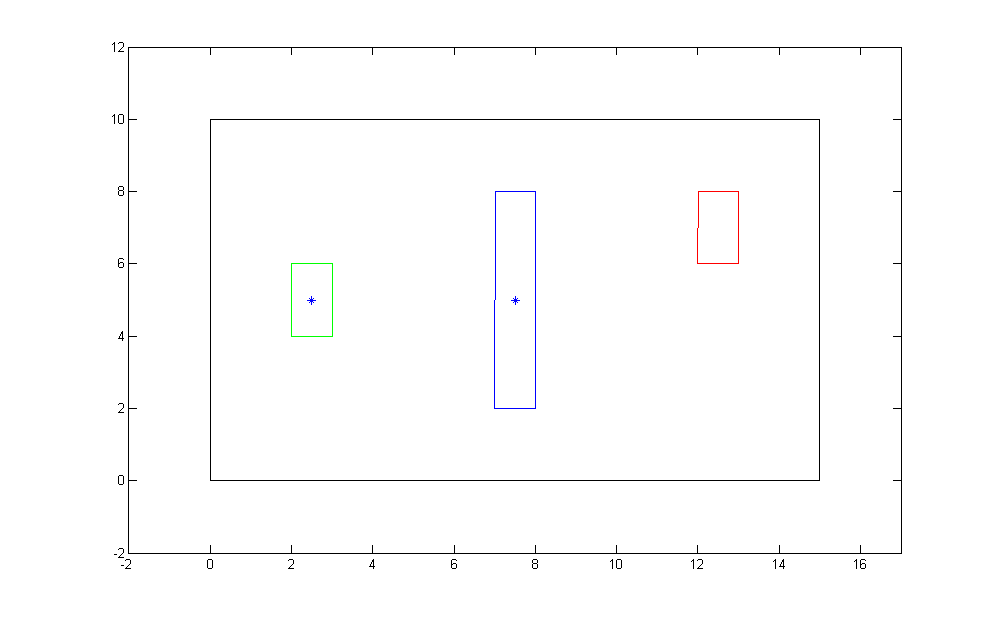
\includegraphics[scale = 0.5]{rotRiddle.png}
\centering
\caption{Riddle with main object, border, target and moveable obstacle.}
\end{figure}
\begin{table}[H]
\centering
\begin{tabular}{l||c|c|c||c|c|c}
& \multicolumn{3}{c||}{rotation} &\multicolumn{3}{c}{translation}\\\hline\hline
Algorithm& fastest & slowest & medium & fastest & slowest & medium\\\hline
pList &  18.8819 & 22.8457  & 21.0269 &  0.1211& 0.1272  & 0.1231\\
fList  & 0.1176&0.1635  &0.1296  & 0.0291 & 0.0504 & 0.0367 \\
fCell & 0.3404 & 0.4012 & 0.3698 & 0.2894 & 0.4112 & 0.3358 \\
\end{tabular}
\caption{Time in seconds for rotation riddle and translation riddle.}
\end{table}

\subsection{Small Riddles}
Two simple small riddles with 2 and 4 moveable obstacles.
\begin{figure}[H]
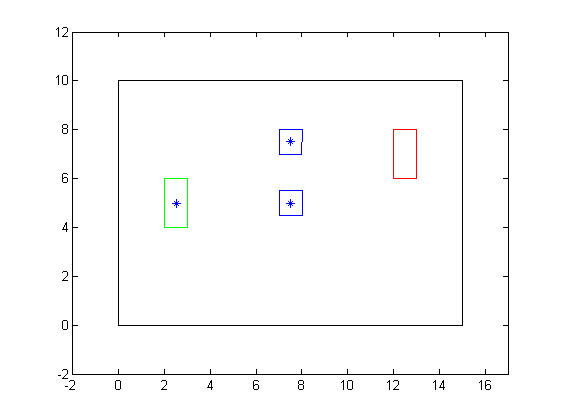
\includegraphics[scale = 0.5]{riddle2}
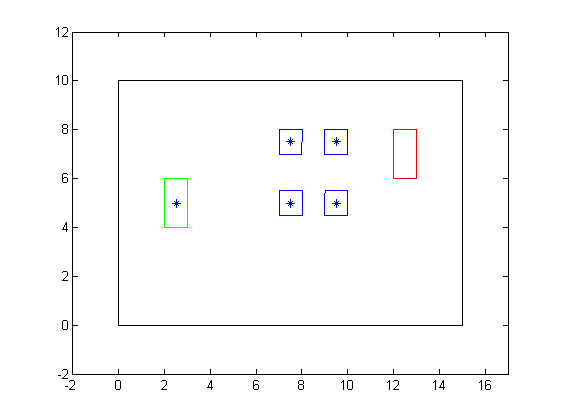
\includegraphics[scale = 0.5]{riddle4}
\caption{Riddle with two and four movable obstacles.}
\end{figure}
\begin{table}[H]
\centering
\begin{tabular}{l||c|c|c||c|c|c}
& \multicolumn{3}{c||}{2 objects} &\multicolumn{3}{c}{4 objects}\\\hline\hline
Algorithm& fastest & slowest & medium & fastest & slowest & medium\\\hline
pList & 4.7801& 5.1930&4.9305& 85.1726 & 90.9629 & 89.3621\\
fList  & 0.6242 & 0.8082& 0.6747  & 7.3608 & 8.1557 & 7.7242\\
fCell & 0.1362 & 0.1591 & 0.1472 & 13.2560 & 14.0114 & 13.5623\\
\end{tabular}
\caption{Time in seconds for small riddle with 2 and 4 obstacles.}
\end{table}
% cell times 2 | 4
% avg 0.1285| 6.2646
% min 0.1267| 6.1976
%max 0.1320| 6.3642

\subsection{Medium Riddles}
Bigger riddle with 6 and 8 moveable obstacles.\\
\begin{figure}[H]
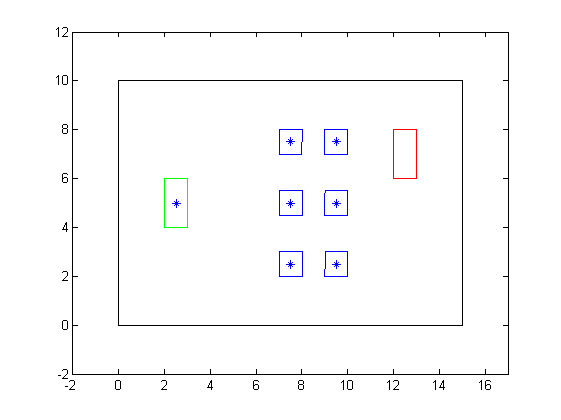
\includegraphics[scale = 0.5]{riddle6}
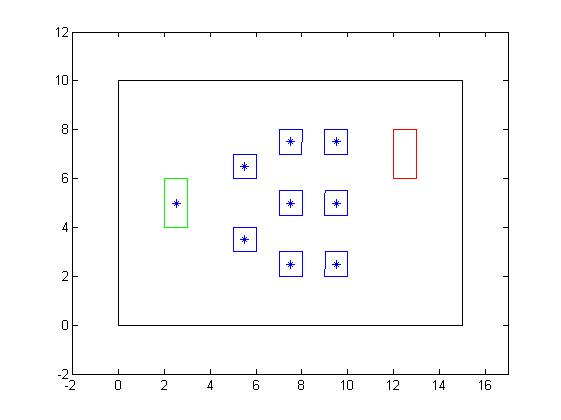
\includegraphics[scale = 0.5]{riddle8}
\caption{Riddle with six and eight moveable obstacles.}
\end{figure}
\begin{table}[H]
\centering
\begin{tabular}{l||c|c|c||c|c|c}
& \multicolumn{3}{c||}{6 objects} &\multicolumn{3}{c}{8 objects}\\\hline\hline
Algorithm& fastest & slowest & medium & fastest & slowest & medium\\\hline
pList &  395.0670 & 415.7986 & 403.9329  & 1790.5 &1972.5 &1855.4\\
fList  &  32.6039 &  34.4411 & 33.7001 & 30.4606 & 33.9077 & 32.1049\\
fCell & 49.1205 & 51.2846 & 50.3155 & 95.5828 & 106.6468 & 100.63497\\
\end{tabular}
\caption{Time in seconds for medium riddle with 6 and 8 obstacles.}
\end{table}

%\subsection{Large riddles}
%Large riddle with 12 and 16 moveable obstacles.\\
%\begin{figure}[H]
%%\includegraphics[scale = 0.5]{riddle12}
%%\includegraphics[scale = 0.5]{riddle16}
%\caption{Riddle with twelve and sixteen moveable obstacles.}
%\end{figure}
%\begin{table}[H]
%\centering
%\begin{tabular}{l||c|c|c||c|c|c}
%& \multicolumn{3}{c||}{12 objects} &\multicolumn{3}{c}{16 objects}\\\hline\hline
%Algorithm& fastest & slowest & medium & fastest & slowest & medium\\\hline
%pList &  - & - & -  & - &- &-\\
%fList  &  32.6039 &  34.4411 & 33.7001 & 30.4606 & 33.9077 & 32.1049\\
%fCell & 251.4319 & 395.3441 & 305.9431 & 79.4915 & 108.6652 & 102.6317\\
%\end{tabular}
%\caption{Time in seconds for medium riddle with 6 and 8 obstacles.}
%\end{table}

\subsection{Counterheuristic Riddles}
This riddle is build to test the search algorithms heuristic in combination cell identification.\\
\begin{figure}[H]
\centering
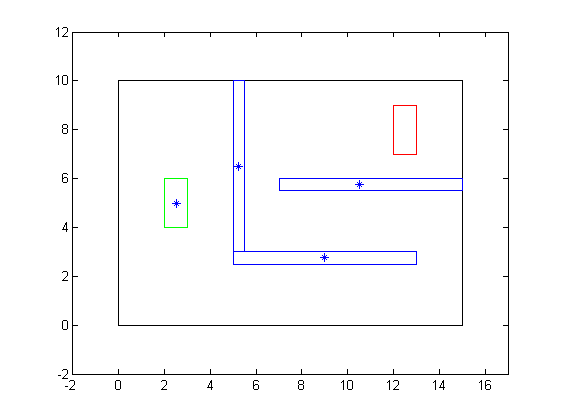
\includegraphics[scale = 0.5]{riddleB}
\caption{Riddle which needs backward step to be solved.}
\end{figure}
\begin{table}[H]
\centering
\begin{tabular}{l||c|c|c}
& \multicolumn{3}{c||}{6 objects} \\\hline\hline
Algorithm& fastest & slowest & medium \\\hline
fList  &  34234 &  35599 & 34917 \\
fList with cells & 24.036 & 27.8225 & 25.001 \\
\end{tabular}
\caption{Time in seconds for counterheuristic riddle.}
\end{table}


%    min 34234
%    max 35599
%    avg 34917
% times for riddleB with function implementation

% min 24.0345
% avg 25.001
% max 27.8225
% time for riddleB with cell function implementation

\section{Interpretation}
As we can see the algorithm working with functions is much faster. But still it scales with an increasing amount of objects to work with.
If we plot these two against each other we see an exponential grow depending on the number of objects involved for the pList algorithm.
The fList algorithms still scale with the number of objects, but are more dependent on the initial positioning of the objects.
\begin{figure}[H]
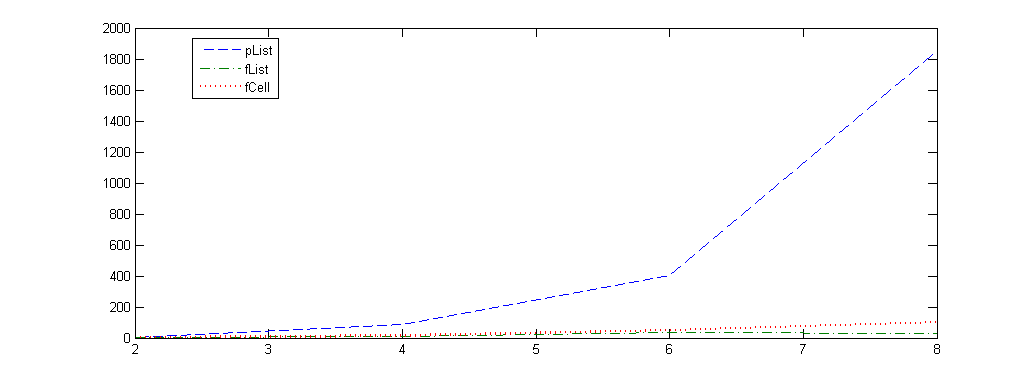
\includegraphics[width=\textwidth]{pointAgainstFuncAgainstCell.png}
\caption{ Plot of the tree algorithms showing the time needed to finish depending on the objects involved.}
\end{figure}
It can easily be seen, that the algorithm pList with point list representation scales extremely bad with an increasing number of objects. This is due to the fact that not only the objects in the direct way beetween target and starting point are considered, but also the extended vectors of objects that are not in the way. This leads to increased number of cells to search through.
\begin{figure}[H]
\centering
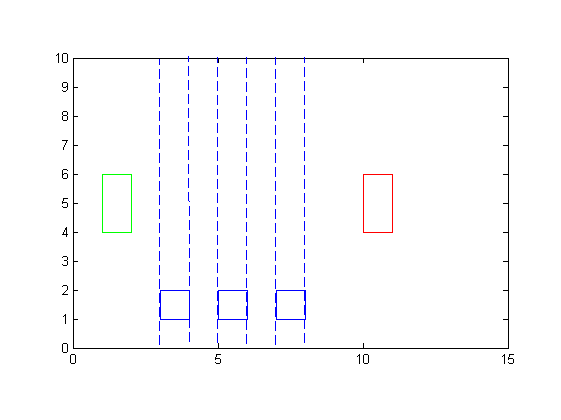
\includegraphics[width=\textwidth, height=250pt]{ghostplanesStep}
\caption{Plot showing the ghostplanes between main object and target.}
\end{figure}
In this plot we can see that there are 6 ghostplanes, extending from the borders of the obstacles in blue, beetween the main object in green and the target in red. Due to this $6\cdot2 = 12$ unnecessary steps need to be calculated before the final step, as per plane we calculate a position in front and behind before evaluating which position is better.\\
If this scenario is given to the algorithm $fList$ ( $fCell$ ) with functions, it would simply check if the obstacles on the bottom are in the way. And as that is not the case, no unecessary steps would arise and the algorithm woud finish in 1 step.\\
\newline
Concerning the counterheuristic riddle the data shows that the algorithm $fCell$ is around $1400$ times faster than the simpler $fList$ algorithm. The algorithm with $pList$ is not listed here, as it takes more than $16h = 57600$ to finish. The calculation was abonded at that time.\\
Comparing the two algorithms $fList$ and $fCel$l, it can be seen that $fList$ is faster for normal calculations with many objects, but fails if the heuristik is bad in the pathplanning. \\
$fCel$l on the other hand reduces the number of cells, thus decreasing the number of steps for the pathplanning. This shortens the path in a way, such that fewer steps in the wrong direction need to be taken to find the target. So for a general purpose algorithm, $fCell$ would be the best choice as it takes only a small penalty for more objects added compared to $fList$, but can deal better with hard riddles.
	\chapterfin

	\chapter{Discussion}
\section{Problems and Solutions}
Through applying a local approach to builing the configuration space, the riddles are starting to become solvable in an acceptable timeframe.
Still, the time it takes to solve a riddle can vary strong depending on the number of objects, their start configuration and their shape. 

\subsection{Invisible plains}
An invisible plain is a plain extending from the vector of one object beetween two of its points. This plain splits the search space in two parts. Due to the fact, that we use this effect to split the space in cells, which we use for nodes in our search graph, changes to these plains affect our graph.\\
%iinsert graphic about two objects with plains interfearing
GRAPHIC WITH TWO OBJECTS PLAINS INTERFEARING\\
If we take a look at this example, we can see how the object o1 dictates the cell border for object o2 on the left. If we move o2 over the border, it now takes over the cell border for object o1. Without a given heuristic which object is better to be moved to the right, this will end in alternating movements for both objects.\\
But if we choose o1 to be the main object, which has a target on the right, the heuristic would need to tell our search algorithm that the point with o1 beeing right of o2 is the better point, and search from there on further, meaning o1 beeing moved to the right cell border again.
GRAPHIC WITH O1 AS MAIN OBJECT???

\subsection{Infinite rotation}
%insert graphic spiral riddle
GRAPHIC WITH A HUGE SPIRAL REQUIERING THE OBJECT TO ROTATE OVER 360° TO SOLVE\\
As earch object can be rotated a total 360° to get back to its starting position, the first thing that comes into mind is that rotations are infinite. The problem with this viewpoint is, that the configuration space would also be infinite in each rotation direction per object. This makes it impossible to calculate the configuration space beforehand, because to do so, each possible combination of objects needs to be checked. But with multiple infinite axis, this would be an infinite number and calculations would never come to an end. \\
The solution to this problem lies in the local search method applied in the algorithm. It views the rotation axis as a stack of configuration hyperplanes per object. If you rotate an arbitrary object o, you simply move up/down in the stack of hyperplanes for said object. \\
The downside to that is, that in order to build a stack, there is the need to define a stepsize in which to move up and down the stack and change the rotation. This leads to another scale factor which needs to be set so that adequate accuracy can be achieved. One has to choose either less accuracy for less calculations or more calculations for higher accuracy.
	\chapterfin

	\chapter{Conclusion}
\section{Applications and Further Usage}
As already noted in \ref{sec:Motivation} there are multiple appliances in the field of robotics and the gaming industry. The exact use is open due to the generalised representation of the problem as a simple riddle to be solved. Thus every practical problem that can be expressed as a geometric riddle in theoretically $n$-dimensional space can be solved with these algorithms.\\
Also there is the possibility to further improve the algorithms. One could allow non-convex moving objects by, for example, representing them as a set of convex objects. Or for algorithm $fList$ with function list representing the rotation not as a set of planes, but as a continuously function which would then give the possibility to check for a collision while rotating and as such removing the need to rotate on a set grid of angles.\\
Another general thing would be a try on implementing the algorithm in a way such that parallel computation is possible. At the moment this would only be possible for each of the $n$ objects movements making the algorithm idealy $n\cdot3\cdot2$ times faster ( 2 translational dimensions and 1 rotational dimension with increasing/decreasing directions ). But as this parallelization depends on the programming language and enviroment used for applying the algorithm it is hard to tell how much of an increase in speed could be obtained.
\section{Summary}
In the creation of this thesis tree algorithms for solving object displacement problems were build, implemented and tested. One as a simple approach with an easy geometric way to understand the representation of world objects and two using an analytic approach making computation easier but losing the simple method of representation. \\
All algorithms showed an improvement if compared to a solution using a fixed grid to calculate all possible combinations of objects involved in both accuracy and speed. Due to the nature of the problem, rotations still propose a big problem which needs to be solved for access to a faster solution. Also all problems are bound to have convex moveable objects only. This need for convex objects could be cut if concave objects are build out of multiple convex objects that move together.\\
From the current data, the algorithm $fCell$ emerged as the all-around best solution to general purpose riddles.This algorithm can be applied to an amount of very different problems, due to the fact that in their core they solve a collision detection problem combined with pathfinding which is needed in many applications.   
	\chapterfin


%---------------------------------------------------------------------------
% Anhang
%---------------------------------------------------------------------------
	\appendix
		
		%---------------------------------------------------------------------------

	\addcontentsline{toc}{chapter}{Resources}

		%---------------------------------------------------------------------------
		\addcontentsline{toc}{section}{List of Figures}
		\listoffigures
		\sectionfin		
		%---------------------------------------------------------------------------
	
		%---------------------------------------------------------------------------
		\addcontentsline{toc}{section}{List of Tables}
		%If you are using e. g. the documentclass book with page style headings you
		%should also take care of correct headings:	
		%\markboth{Abk�rzungsverzechnis}{Abk�rzungsverzechnis}
		\listoftables	
		\printnomenclature
		\sectionfin
		%---------------------------------------------------------------------------
	
		%---------------------------------------------------------------------------
		\nocite{Zitat}
		%---------------------------------------------------------------------------
		\renewcommand\bibname{Bibliography}
		\addcontentsline{toc}{section}{Bibliography}
		\bibliographystyle{acm}
		\bibliography{bibliography}

		\chapterfin

\end{document}
